\section{Theory}
\subsection{The Fabry-Perot interferometer}\label{sec:fabry_perot}

The Fabry-Perot interferometer, also known as an optical cavity, is generally comprised of two reflective optical elements, hereafter referred to as mirrors. In the following we assume a plane-plane configuration for two lossless mirrors and a plane-wave at normal incidence for the incoming field, as sketched in figure \ref{fig:planar_fabry-perot}. 

\begin{figure}[h!]
    \centering
    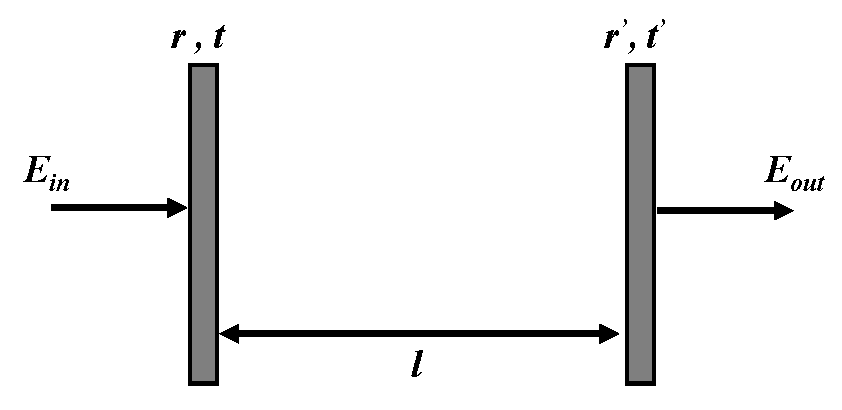
\includegraphics[width=0.6\textwidth]{figures/planar_fabry_perot.pdf}
    \caption{Schematics of a planar Fabry-Perot cavity.}
    \label{fig:planar_fabry-perot}
\end{figure}

The two mirrors are described by each their respective amplitude coefficients for the reflectivity \emph{r} and transmission \emph{t} and are placed parallel at a distance \emph{l} from each other. The field at the second mirror, i.e. the transmitted field $E_{out}$ can then be described as a function of the field at the first mirror, i.e. the incident field $E_{in}$\cite{Eichhorn,Pedrotti}. 

\subsubsection{Transmission}

In order to determine the transmission through the Fabry-Perot cavity, we once again consider the configuration in figure \ref{fig:planar_fabry-perot}. It is further assumed that the mirrors are both lossless, such that
\begin{equation}
    |r|^2 + |t|^2 = |r^{\prime}|^2 + |t^{\prime}|^2 = 1.
    \label{eq:lossless_condition}
\end{equation}

This means that all losses, e.g. due to absorption or scattering, are neglected. 

In order to formulate $E_{out}$ in terms of $E_{in}$, we first consider the incident field as a propagating plane-wave with wave number $k = 2 \pi / \lambda$. We then consider $E_{out}$ to be comprised of contributions for each roundtrip inside the cavity. This can be written as an infinite geometrical series given as
\begin{equation}
    \begin{split}
        E_{out} & = tt^{\prime} E_{in} e^{ik \delta / 2} + tt^{\prime} E_{in} e^{ik \delta / 2} rr^{\prime} e^{i\delta}\\&+ tt^{\prime} E_{in} e^{ik \delta / 2} \left(rr^{\prime} e^{i\delta}\right)^2 + tt^{\prime} E_{in} e^{ik \delta / 2} \left(rr^{\prime} e^{i\delta}\right)^3 + ...\\& = tt^{\prime} E_{in} e^{ik \delta / 2} \sum^{\infty}_{m=0}\left( rr^{\prime}e^{i\delta} \right)^m
    \end{split}
    \label{eq:transmission_as_geometric_series}
\end{equation}
where $\delta = 2kl$. The first term of the series corresponds to a direct transmission through the cavity, and each term thereafter corresponds to the respective contribution to the transmission after the $m'th$ round trip. 

By evaluating the series it is seen that it converges to the final expression for the transmitted field through a planar Fabry-Perot cavity
\begin{equation}
    E_{out} = E_{in}\frac{tt^{\prime} e^{i\delta /2}}{1 - rr^{\prime} e^{i\delta}}.
    \label{eq:fabry_perot_trans}
\end{equation}

The intensity of the transmission is now taken as the square of the norm of the field intensity $|E_{out}|^2$ and normalizing with respect to the incident field intensity $|E_{in}|^2$. We arrive at an expression for the transmission intensity which is an \emph{Airy function}\cite{Pedrotti}
\begin{equation}
    T = \frac{|E_{out}|^2}{|E_{in}|^2} = \left|\frac{tt^{\prime}e^{i\delta/2}}{1 - rr^{\prime}e^{i \delta}}\right|^2 = \frac{(1-|r|^2)(1-|r^{\prime}|^2)}{(1-|rr^{\prime}|)^2 + 4|rr^{\prime}|sin^2(\delta)},
    \label{eq:airy_function}
\end{equation}
where $\delta$ is the phase shift associated with each round trip inside the cavity.

\begin{figure}[h!]
    \centering
    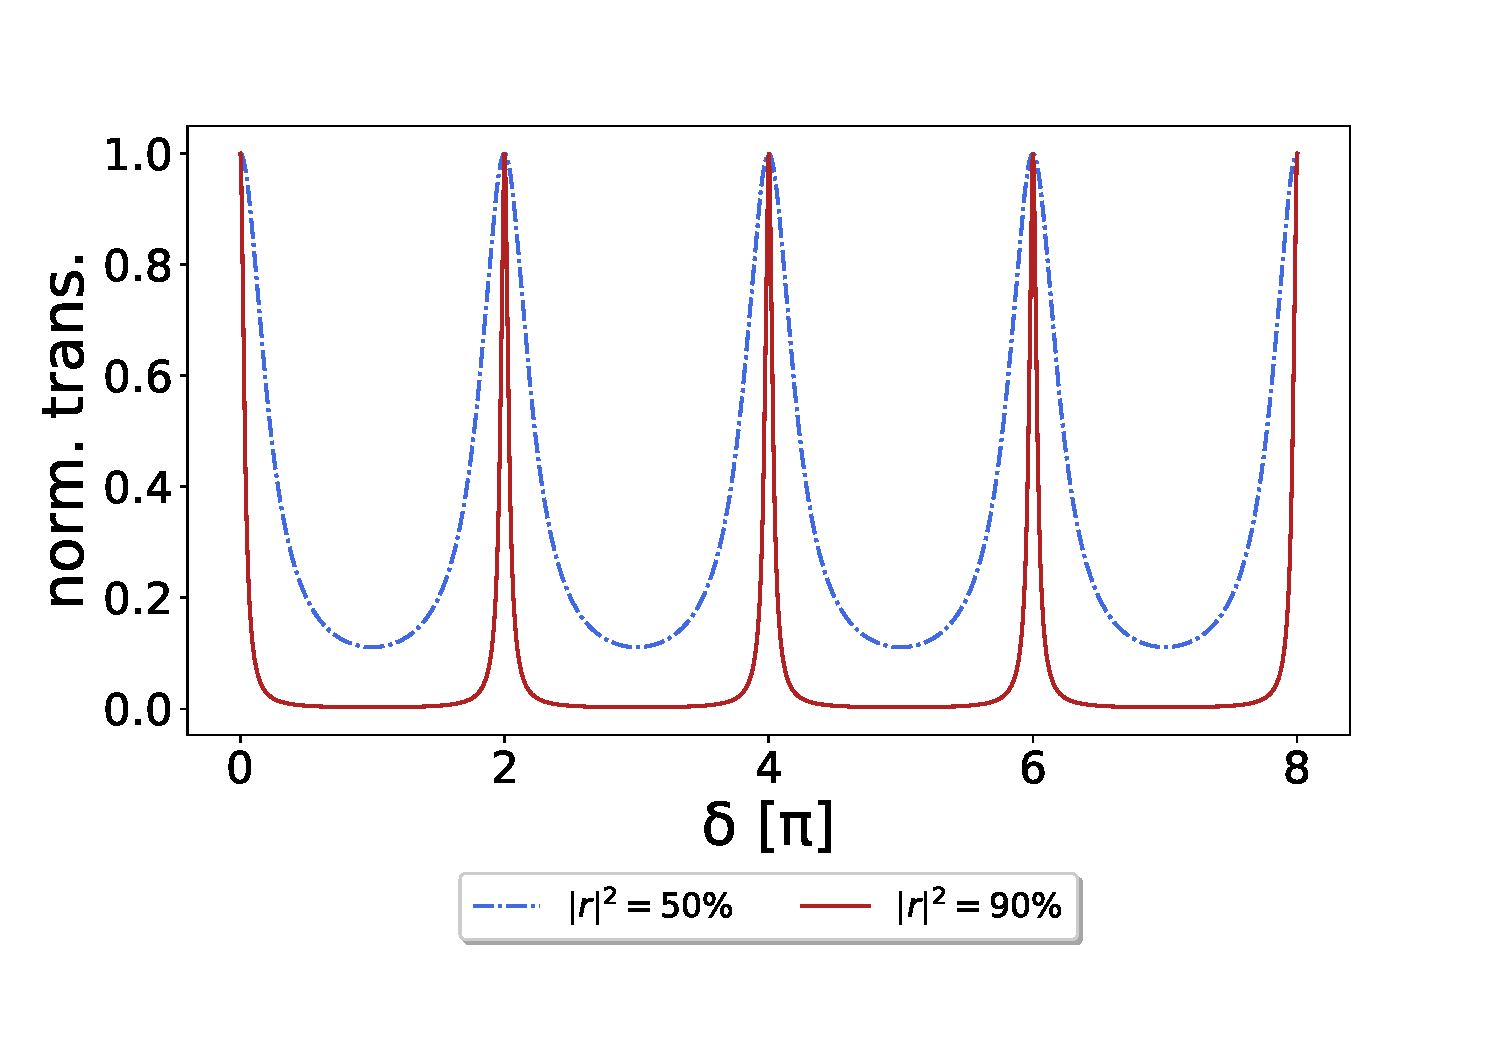
\includegraphics[width=0.7\textwidth]{figures/fabry_perot_high_and_low_finesse.pdf}
    \caption{The red line shows the transmission spectrum of a high finesse Fabry-Perot cavity of reflectivity $|r|^2 = 0.90$, while the blue dashed line shows the transmission spectrum of a low finesse cavity with reflectivity $|r|^2 = 0.50$.}
    \label{fig:fabry_perot_trans}
\end{figure}

Figure \ref{fig:fabry_perot_trans} displays the Airy function in eq. (\ref{eq:airy_function}), of a lossless cavity with mirrors of equal reflectivities $r^{\prime} = r$, as a function of $\delta$ in units of $\pi$. The function is plotted for the cases of $|r|^2 = 50 \%$, shown in blue, and $|r|^2 = 90 \%$, shown in red. It is readily seen that the transmission is maximized for $\delta = n 2 \pi$, which corresponds to standing wave modes with $\lambda_n = 2l/n$. It is further seen that the two cases shown differ significantly as the red profile is much narrower than the blue. The red profile is hence said to have a higher \emph{finesse} $\mathcal{F}$ than the blue profile. The finesse is a measure of the quality of a cavity by the distance between succesive resonance peaks relative to their width. It is thus defined as
\begin{equation}
    \mathcal{F} \equiv \frac{FSR}{\delta_{\lambda}},
    \label{eq:finesse_definition}
\end{equation}
where $FSR$ is the so-called \emph{Free Spectral Range} indicating the spectral distance between two peaks and $\delta_{\lambda}$ refers to the \emph{Full Width at Half Maximum (FWHM)} which, as the name suggests, is the linewidth defined at half the maximum value for the normalized transmission.

Considering the Airy function in eq. (\ref{eq:airy_function}) for the high finesse case where $|r|^2 = |r^{\prime}|^2 \rightarrow 1$ we furthermore see that each individual peak closely resembles a Lorentzian function. 

Note here that the field intensity inside the cavity is closely related to the Fabry-Perot transmission function, this is denoted the so-called \emph{intracavity} intensity. It is representative of the field build-up inside the cavity and is defined as 
\begin{equation}
    |E_{cav}|^2 \equiv |E_{in}|^2 \left|\frac{1}{1-rr^{\prime}e^{i\delta}}\right|^2.
    \label{eq:intracavity_intensity}
\end{equation}

\subsubsection{Varying the cavity length}

In order to relate the resonance transmission profile to the length of the cavity we first consider the frequencies at which the cavity is resonant, with respect to the incident light, given as
\begin{equation}
    \nu_n = n \frac{c}{2l},
    \label{eq:resonance_freq}
\end{equation}
where $c$ is the speed of light, $n$ is a positive integer referring to the order of the resonance frequency and $l$ is the cavity length. This corresponds to resonance occuring at times related to each round trip inside the cavity. 

Since the FSR is defined as the spectral distance between each peak, it follows from eq. (\ref{eq:resonance_freq}) that it can be expressed in units of frequency as 
\begin{equation}
    FSR_{\nu} = \frac{c}{2l},
    \label{eq:FSR_vs_cavity_length}
\end{equation}
and the corresponding linewidth, or FWHM, $\delta_{\nu}$ is then given as
\begin{equation}
    \delta_{\nu} = \frac{1}{2 \pi} \frac{|t|^2 + |t^{\prime}|^2}{\tau},
\end{equation}
where $\tau = 2l/c$ is the round trip time in seconds. 

Finally, considering the definition of the finesse from eq. (\ref{eq:finesse_definition}) it can be shown that
\begin{equation}
    \mathcal{F} \equiv \frac{FSR_{\nu}}{\delta_{\nu}} = \frac{2 \pi}{|t|^2 + |t^{\prime}|^2},
    \label{eq:lossless_finesse}
\end{equation}
where the finesse is now defined in terms of the total cavity transmission at resonance. 

Note here that the relation between the FSR and the cavity length $l$ is clearly shown in eq. (\ref{eq:FSR_vs_cavity_length}), and figure \ref{fig:fabry_perot_FSR_comparison} furthermore shows transmission spectra highlighting the effect of changing the cavity length. 

\begin{figure}[h!]
    \centering
    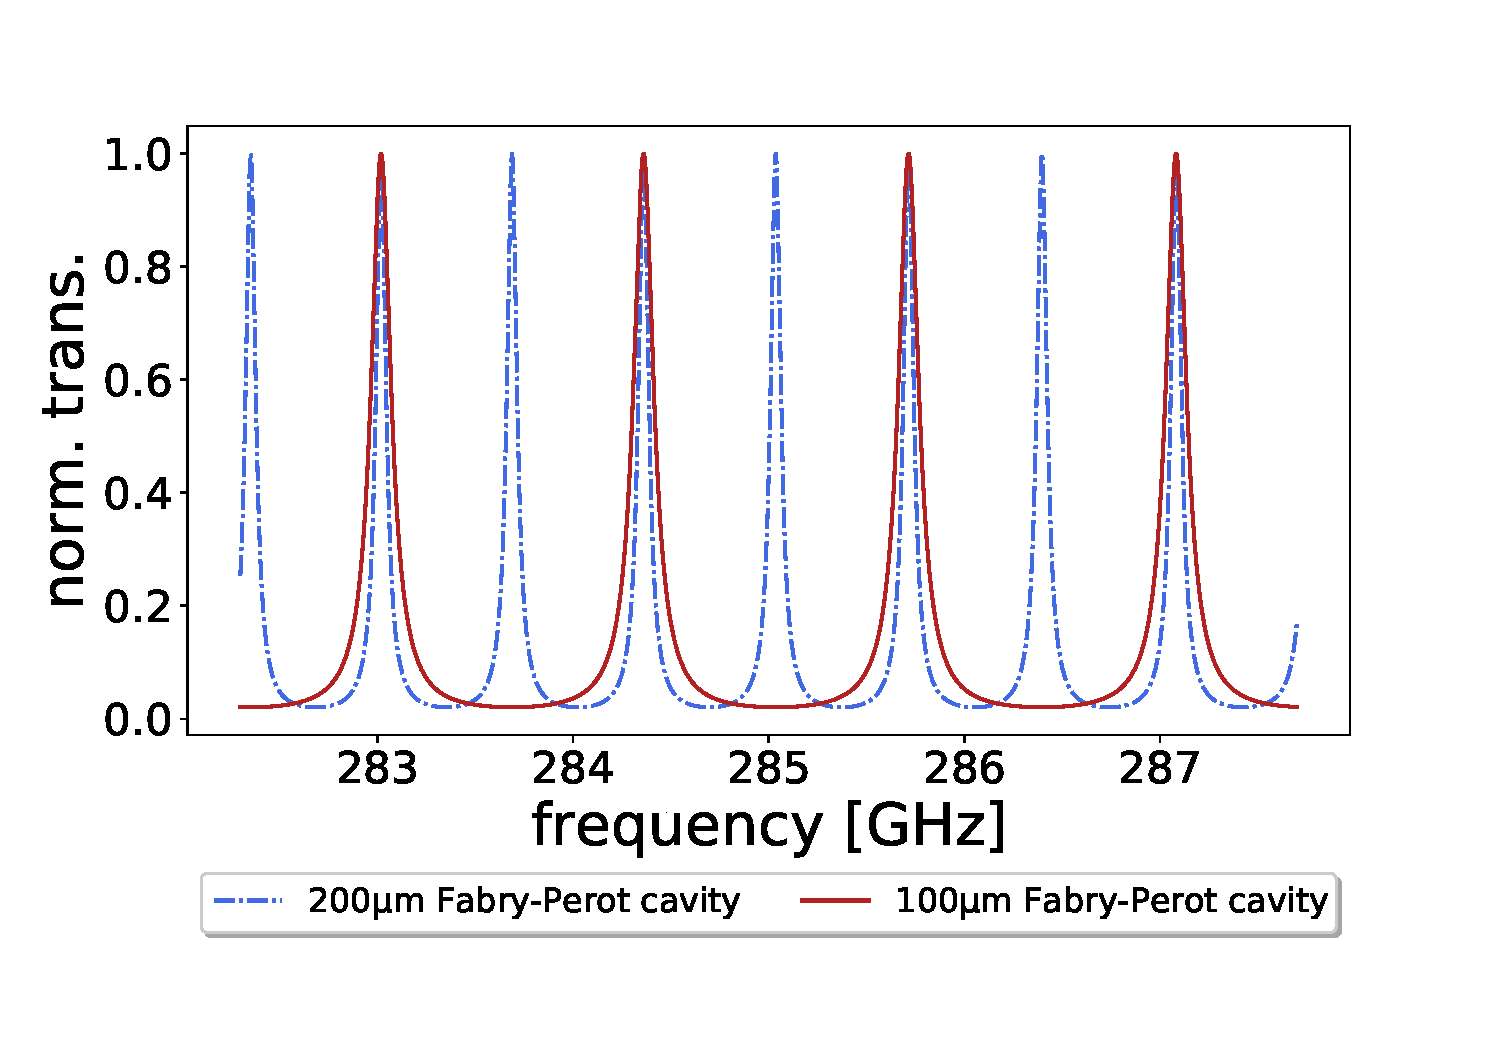
\includegraphics[width=0.7\textwidth]{figures/100um_and_200um_fabry_perot_trans_vs_freq.pdf}
    \caption{Fabry-Perot transmission spectra for cavities of lengths $l = 100 \mu m$ and $l = 200 \mu m$. It is clearly seen that the FSR is inversly proportional with the cavity length as it is apparent that $FSR_{100 \mu m} = 2 \cdot FSR_{200 \mu m}$.}
    \label{fig:fabry_perot_FSR_comparison}
\end{figure}

\subsubsection{Varying the incident wavelength}

In order to simplify the Airy function in eq. (\ref{eq:airy_function}) we introduce the so-called \emph{coefficient of finesse} $F$, which is a function only of the mirror reflectivites, given as
\begin{equation}
    F = \frac{4 |rr^{\prime}|}{(1-|rr^{\prime}|)^2}.
\end{equation}

The coefficient of finesse $F$ is not to be confused with the finesse $\mathcal{F}$, as they are not equal, but rather related by
\begin{equation}
    \mathcal{F} = \frac{\pi}{2} \sqrt{F}.
\end{equation}

Rewriting the Airy function in terms of the coefficient of finesse yields
\begin{equation}
    T_{\lambda} = \frac{1}{1+ F sin^2 \left(\delta / 2\right)},
    \label{eq:simplified_airy_function}
\end{equation}
where the round trip phase shift $\delta$ is related to the wavelength $\lambda$ of the incident light by
\begin{equation}
    \delta = 2kl = \frac{4 \pi l }{\lambda},
\end{equation}
as $k = 2 \pi / \lambda$ is the incident wave number.

Re-writing the general cavity brightness condition, it can easily be shown that the resonant wavelengths for a cavity at normal incidence are given as
\begin{equation}
    \lambda_n = \frac{2l}{n},
\end{equation}
where $n=1,2,3,...$ is a positive integer referring to the order of the resonance. 

Since $\nu = c / \lambda$, the relation between the linewidth in wavelength space $\delta_{\lambda}$ and the one in frequency space $\delta_{\nu}$ is non-linear. Therefore, one does not simply make the aforementioned substitution in order to relate them. However, it can be shown that their respective expressions differ by a factor of $\lambda^2/c$, and the linewidth when varying the wavelength is thus given as
\begin{equation}
    \delta_{\lambda} = \frac{\lambda^2}{c} \cdot \delta_{\nu} = \frac{\lambda^2}{4 \pi l} (|t|^2 + |t^{\prime}|^2).
\end{equation}
Finally, we consider the definition for the finesse $\mathcal{F}$ and the expression given in eq. (\ref{eq:lossless_finesse}), in order to show that the $FSR$ in wavelength space is given as 
\begin{equation}
    FSR_{\lambda} \equiv \delta_{\lambda} \cdot \mathcal{F} =  \frac{\lambda^2}{2l}.
\end{equation}
Figure \ref{fig:airy_trans_vs_wavelength} shows an example of the Airy function given in eq. (\ref{eq:simplified_airy_function}) as a function of the wavelength for a lossless Fabry-Perot cavity of reflectivity intensites $|r|^2 = |r^{\prime}|^2 = 90\%$, transmission intensities $|t|^2 = |t^{\prime}|^2 = 10\%$ and length $l=100 \mu m$. It also includes an example of the transmission function with non-zero cavity losses, this is outlined further in section \ref{sec:cavity_losses} below.

\begin{figure}[h!]
    \centering
    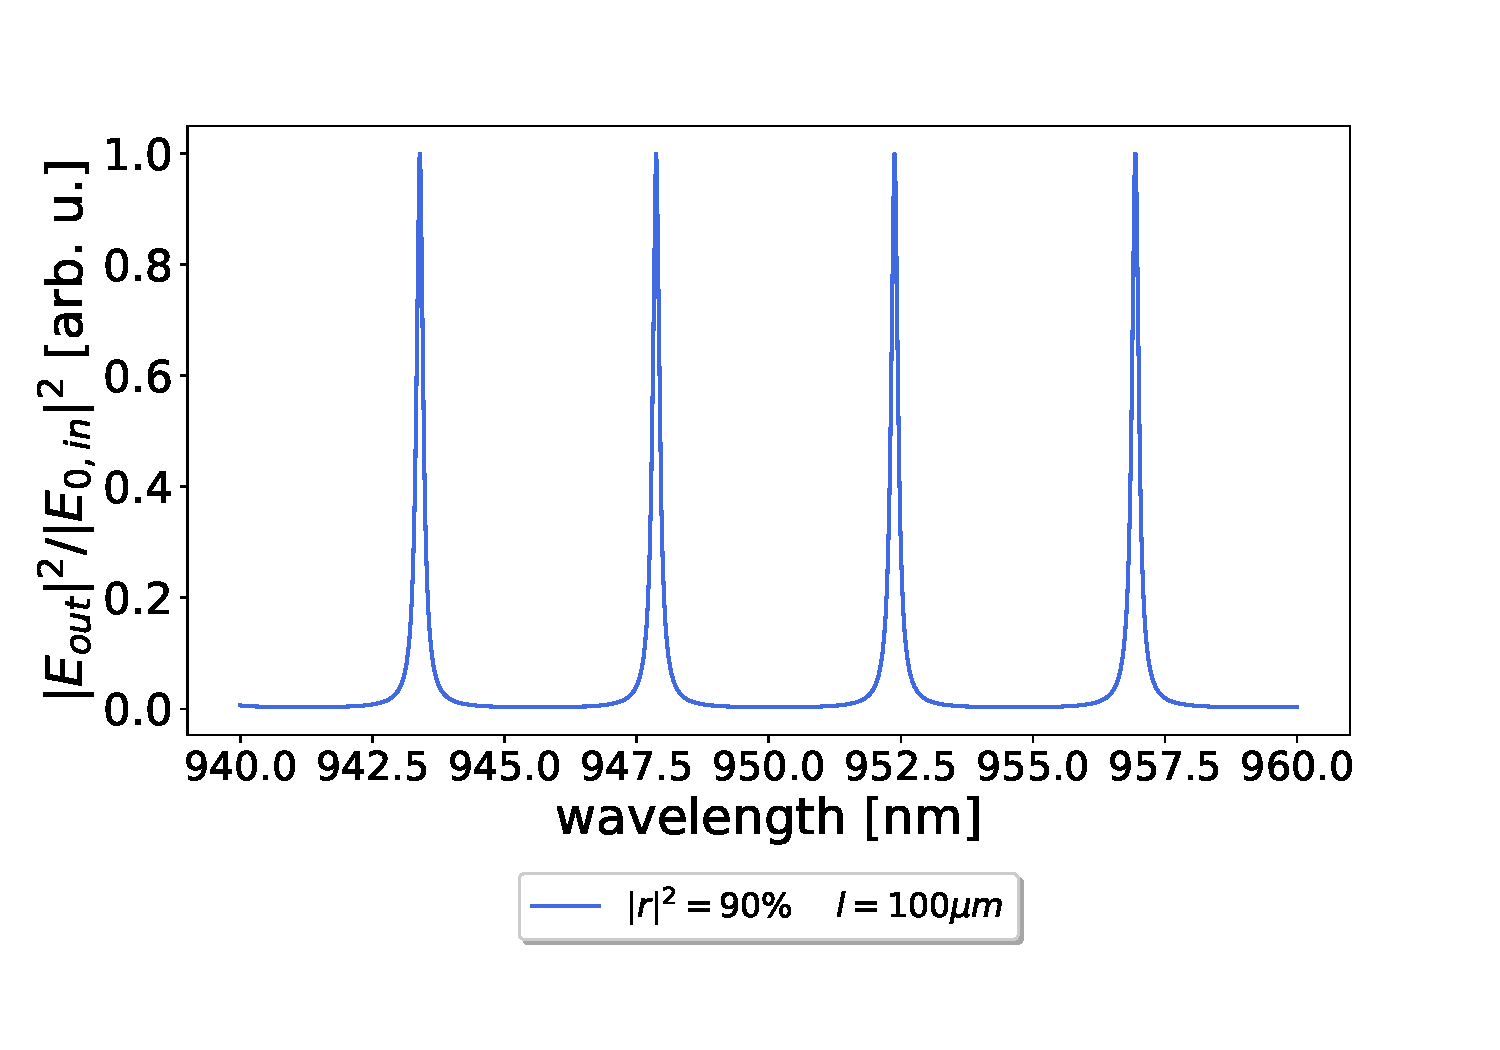
\includegraphics[width=0.7\textwidth]{figures/airy_function_vs_wavelength.pdf}
    \caption{The Airy function as seen in eq. (\ref{eq:simplified_airy_function}), plotted as a function of the incident wavelength for a cavity length of $l = 100 \mu m$. The blue dashed line shows an example without losses due to e.g. scattering or absorption, while the red line shows an example of a lossy cavity with intensities given as $|r|^2 = 70\%$, $|t|^2 = 10\%$ and $L = 20\%$.}
    \label{fig:airy_trans_vs_wavelength}
\end{figure}

\subsubsection{Cavity losses}\label{sec:cavity_losses}

In eq. (\ref{eq:lossless_finesse}), we assume the case of a lossless cavity, i.e. eq. (\ref{eq:lossless_condition}) is fulfilled. In practice, any cavity will have some amount of losses, which would have to be taken into account when calculating the finesse. When losses are present, eq. (\ref{eq:lossless_condition}) instead generally reads
\begin{eqnarray}
    |r|^2 + |t|^2 + L + L^{\prime} = 1,
\end{eqnarray}
where $L$ and $L^{\prime}$ indicate the fractional losses of each mirror.

In this case the finesse would be given as 
\begin{equation}
    \mathcal{F} = \frac{2 \pi}{|t|^2 + |t^{\prime}|^2 + L_{total}},
\end{equation}
where $L_{total} = L + L^{\prime}$ is the total additional cavity losses.

The effect on the transmission spectrum of a cavity with losses is that the level of the normalized transmission will not reach unity, as some light is lost to e.g. absorption or scattering for each round trip of the cavity. This is shown in figure \ref{fig:airy_trans_vs_wavelength} where the Airy function is shown and compared for examples with $L=0$ and $L=20\%$.
